\documentclass{beamer}
\usetheme{default}

\usepackage{graphicx}
\graphicspath{{../../images/}}

\setbeamertemplate{caption}[numbered]

\title{Chapter-04: Model-View-ViewModel (MVVM) Architecture}
\subtitle{IF231303-Software Architecture\\Pradita University}
\author{Alfa Yohannis}
\begin{document}

\begin{frame}[plain]
    \maketitle
\end{frame}

\begin{frame}{Model-View-ViewModel Schema}
\begin{figure}[h]
    \centering
    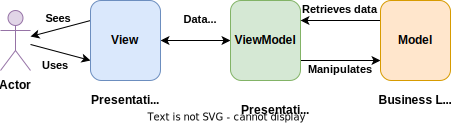
\includegraphics[width=\textwidth]{mvvm}
    \caption{Model-view-viewmodel (MVVM) architecture.}
    \label{fig:mvvm}
\end{figure}
\end{frame}

\begin{frame}{Background}
\begin{itemize}
\item In the beginning, software development put the functions of graphical user interface (GUI) and data management into one code, with no separation of concerns.
\item MVC pattern then emerged to separate the concerns related to views, presentation \& business logics, models. However, there were no explicit abstraction that maintains the states of views.  
\item MVP addressed it that the \texttt{Presenter} managed the presentation logic of views.
Nevertheless, the code that maintain the synchronisation of the views and the states of their presentation logics have to be crafted manually.
\item Model-View-ViewModel has a binder that automates communication between the view and its bound properties in the view model, reducing the need to write boiler-plate logic to synchronise -- send and receive updates -- the view model and view.
\end{itemize}
\end{frame}

\begin{frame}{Model-View-ViewModel (MVVM)}
\begin{itemize}
\item One of the architectural patterns for developing Graphical User Interface (GUI) which divides program logic into three interconnected components: Model, View, and ViewModel.
\item \textbf{Model} manages the data and business logics of the application.
\item \textbf{View} is the presentation that users can see and interact with, e.g., webpages, desktop GUI, charts, buttons, text fields, etc.
\item \textbf{ViewModel} is an abstraction of the state of a view exposing public properties. 
\item The presenter in the MVP has a reference to a view, whereas the view model does not. 
\item A view directly binds to properties on the view model to send and receive updates.
\item \textbf{Binder} frees the developer from being obliged to write boiler-plate logic to synchronise the view model and view.  

\end{itemize}
\end{frame}

\begin{frame}{Advantages}
The advantages of MVVM are:
\begin{itemize}
\item Separation of the view layer by moving all GUI code to the view model via data binding.
\item UI developers don't write the the GUI, instead a markup language is used.
\item The separation of roles allows UI designers to focus on the UX design rather than programming of the business logic. 
\item A proper separation of the view from the model is more productive, as the user interface typically changes frequently and late in the development cycle based on end-user feedback.
\item Data bindings and properties are used to synchronise the relevant values in the view and the view model, that represents the state of the view, so that they are always the same.
\item It eliminates or minimises application logic that directly manipulates the view. 

\end{itemize}
\end{frame}

\begin{frame}{Disadvantages}
\begin{itemize}
\item It can be overkill for small projects. 
\item Generalizing the viewmodel upfront can be difficult for large applications.
\item Large-scale data binding can lead to lower performance.
\item It's best for UI development but might not the best for other types of developments and  applications.
\end{itemize}
\end{frame}

\begin{frame}{Other MVVM Variants}
\begin{itemize}
\item Model-View-Presenter (MVP).
\item Model-View-Controller (MVC).
\item Model-View-Adapter (MVA).
\item Hierarchical Model-View-Controller (HMVC).

\end{itemize}
\end{frame}

\end{document}
